\subsection{Geometries}
\label{sect:ImplementedProblems_Geometries}

In the following we give an overview about the geometries which are already available. For adding a new geometry create a new directory \code{<newGeometry>} in \path{./problems/geometries/}. There you have to define the coordinates of the geometry in \path{<newGeometry>_c4n.dat}. The nodes for each triangle have to be defined in \path{<newGeometry>_n4e.dat}. The Dirichlet- and Neumann-part of the domain boundary is specified in \path{<newGeometry>_Db.dat} and \path{<newGeometry>_Nb.dat} respectively.

\begin{figure}[h!]
\includegraphics[width=0.15\textwidth]{images/sect_ImplementedProblems_Triangle.pdf}
\includegraphics[width=0.15\textwidth]{images/sect_ImplementedProblems_Square.pdf}
\includegraphics[width=0.15\textwidth]{images/sect_ImplementedProblems_Lshape.pdf}
\includegraphics[width=0.15\textwidth]{images/sect_ImplementedProblems_Lshape3.pdf}
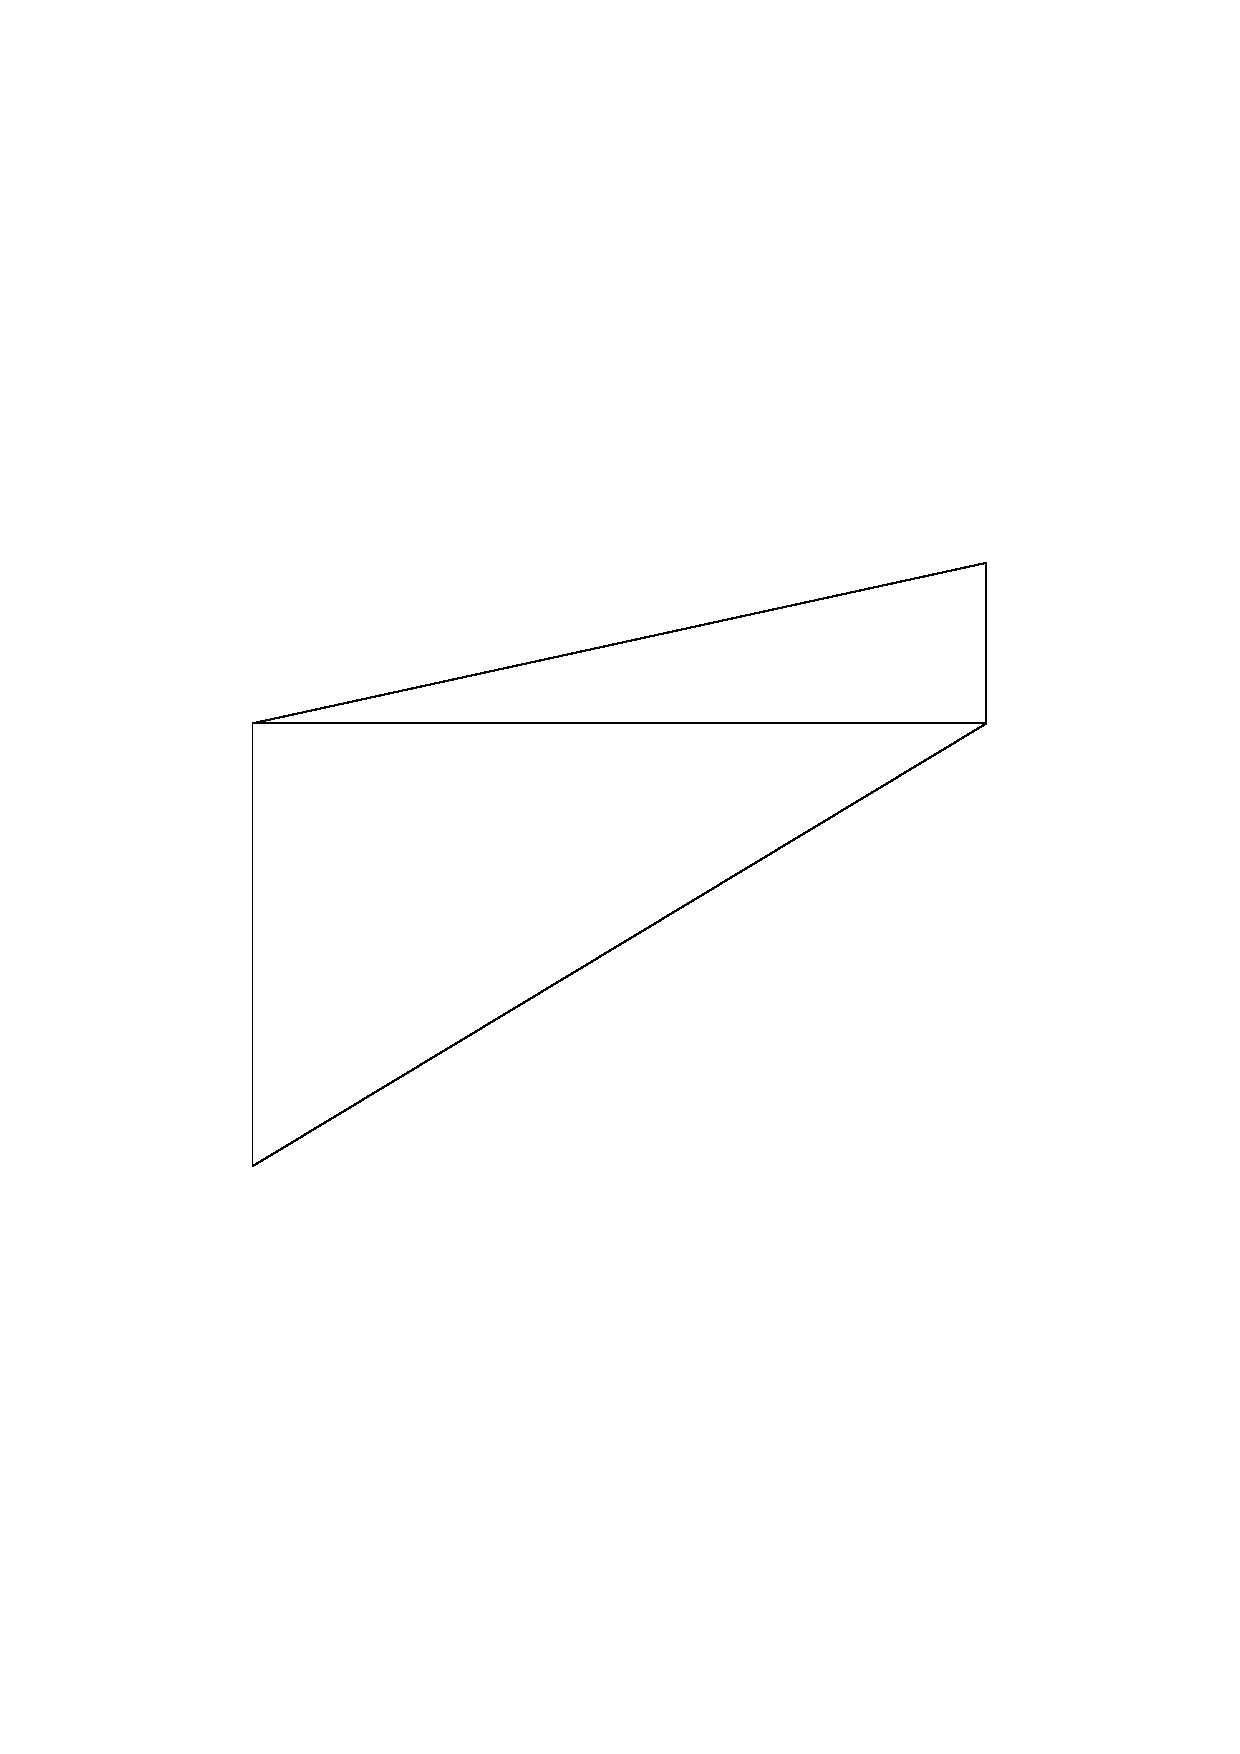
\includegraphics[width=0.15\textwidth]{images/sect_ImplementedProblems_Cooks.pdf}
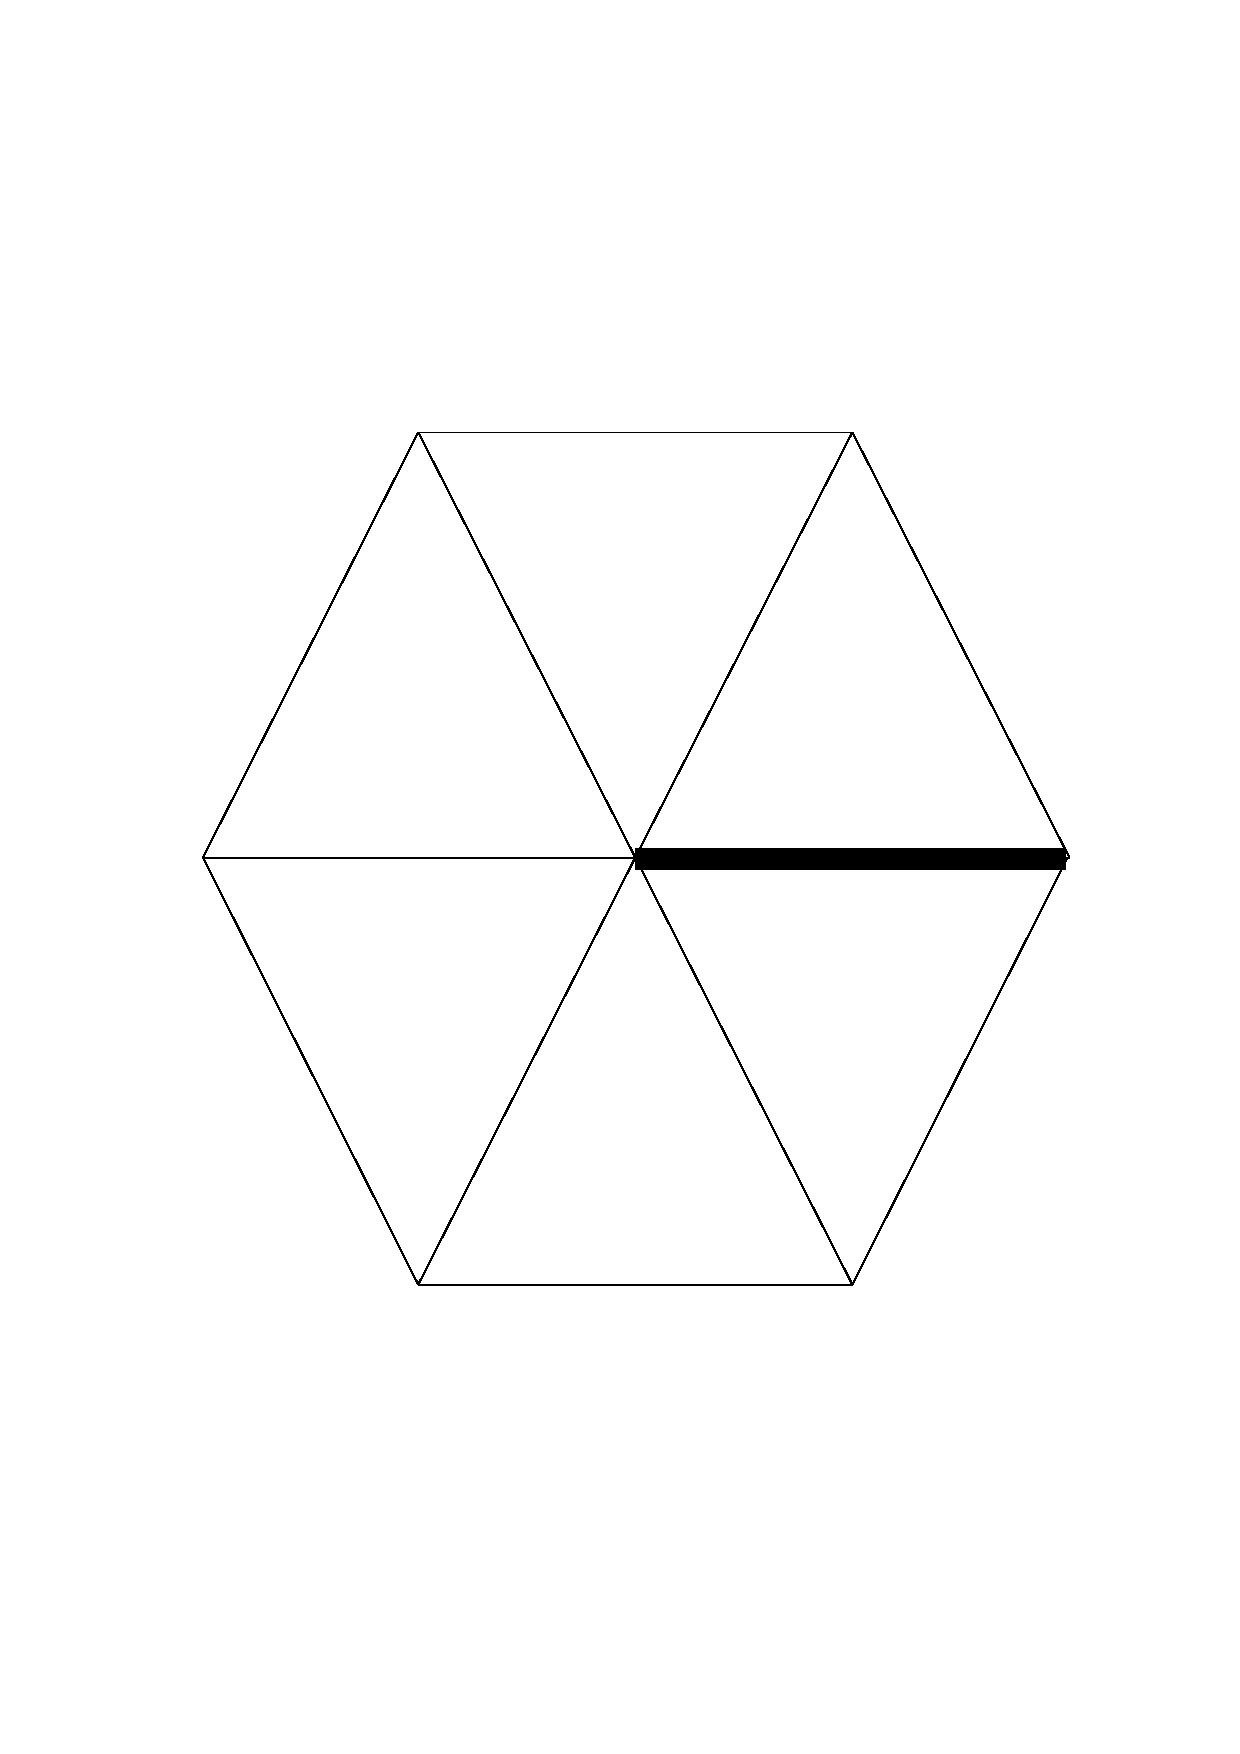
\includegraphics[width=0.15\textwidth]{images/sect_ImplementedProblems_HexagonalSlit.pdf}
\caption{Initial triangulation of implemented geometries. From left to right: Triangle, Square, Lshape, Lshape3, Cooks, HexagonalSlit}
\end{figure}

\begin{tabular}{p{0.25\textwidth}p{0.65\textwidth}}
Geometry Name 	& 	Description \\
\hline
Triangle				& The reference triangle $\Omega=\conv\{(0,0),(1,0),(0,1)\}$ with pure Dirichlet-boundary.\\
Square					& The unit square $\Omega=[0,1]^2$ with pure Dirichlet-boundary.\\
SquareNeumann		& The unit square with Neumann boundary $\Gamma_N=\conv\{(1,0),(1,1)\}$.\\
Lshape          & The L-shaped domain $\Omega=[-1,1]^2\setminus\{(0,1]\times(0,-1]\}$ with pure Dirichlet-boundary.\\
LshapeNeumann		& The domain is the L-shape domain with Neumann boundary.  $\Gamma_D=\left\{\conv\{(0,0),(1,0)\}\cup\conv\{(0,0),(0,-1)\}\right\}$.\\
Lshape3         & Lshape3 is a rotated version of Lshape. Here the boundary of the rotated L-shaped domain is not axis parallel anymore.\\
Lshape3Neumann  & Lshape3Neumann is a rotated version of LshapeNeumann.\\
Cooks						& Geometry for the Cook's membrane problem in elasticity. $\Omega=\conv\{(0,0),(48,44),(48,60),(0,44)\}$. The Dirichlet boundary $\Gamma_D$ is $\conv\{(0,0),(0,44)\}$. Thus the Neumann boundary is $\partial\Omega\setminus\Gamma_D$.\\
HexagonalSlit   & We have defined a hexagon $\Omega\subset[-1,1]^2$ which is slitted in $\{0\}\times[0,1]$. The slit is approximated by adding an additional node through a small, numerically insignificant, perturbation of the node $(0,1)$. The slitted hexagon is an example for a non-Lipschitz domain with pure Dirichlet boundary.
\end{tabular}
